\documentclass[a4paper, 11pt]{article}


\usepackage[slovak]{babel}
\usepackage[utf8]{inputenc}
\usepackage[left=2cm, top=3cm, text={17cm, 24cm}]{geometry}
\usepackage{times}
\usepackage{verbatim}
\usepackage{enumitem}
\usepackage{graphicx} 
\usepackage[unicode]{hyperref}
\usepackage{listings}
\usepackage{color}

\definecolor{dkgreen}{rgb}{0,0.6,0}
\definecolor{gray}{rgb}{0.5,0.5,0.5}
\definecolor{mauve}{rgb}{0.58,0,0.82}

\lstset{language=SQL,
  aboveskip=3mm,
  belowskip=3mm,
  showstringspaces=false,
  columns=flexible,
  basicstyle={\small\ttfamily},
  numbers=none,
  numberstyle=\tiny\color{gray},
  keywordstyle=\color{blue},
  commentstyle=\color{dkgreen},
  stringstyle=\color{mauve},
  breaklines=true,
  breakatwhitespace=true,
  tabsize=3
}



\begin{document}

	\begin{titlepage}
		\begin{center}
			\Huge
			\textsc{Vysoké učení technické v~Brně} \\
			\huge
			\textsc{Fakulta informačních technologií} \\
			\vspace{\stretch{0.382}}
			\LARGE
			Projektová dokumentácia k~predmetu IDS \\
			\Huge
			Zadanie č. 33 - Lékárna
			\vspace{\stretch{0.618}}
		\end{center}

		{\Large
			\today
			\hfill
			\begin{tabular}{r}
			Dávid Oravec (xorave05) \\
			Dominik Boboš (xbobos00)
			\end{tabular}
		}
	\end{titlepage}
	\newpage
	\section{Zadanie}
	Vaším úkolem je vývoj IS lékárny. Lékárna vydává občanům léky jak na předpis, tak za hotové. U~léků vydávaných na předpis může část ceny hradit zdravotní pojišťovna. Některé léky se vydávají pouze na předpis. Systém musí umožnit evidenci vydávaných léků, import příspěvků na léky od zdravotních pojišťoven (může se čas od času měnit), musí poskytovat export výkazů pro zdravotní pojišťovny a musí mít vazbu na skladové zásoby (vidět, zda požadovaný lék je na skladě). Léky jsou identifikovány číselným kódem či názvem.
	\section{Implementácia}
	\subsection{Úvod}
	\par Naša implementácia začala vytvorením tabuliek, ktoré odzrkadlovali návrh v~podobe ER diagramu. Nasledovalo určenie primárnych kľúčov tabuliek, cudzích kľúčov a vytváranie tabuliek, ktoré zobrazovali vzťahy medzi entitami v~ER diagrame. Po vytvorení tabuliek sme ich naplnili ukážkovými dátami. Dáta o~lekárňach a liekoch sme čerpali zo strániek lekární. \\
	\par Ďalšou fázou bolo vytvorenie SELECT dotazov. Uvedieme len niekoľko príkladov, ostatné dotazy sú popísané v~kóde.
	\subsubsection{Spojenie 2 tabuliek príkazom SELECT}
	 \begin{lstlisting}
    SELECT *
        FROM LEKAREN NATURAL JOIN ZDRAVOTNA_POISTOVNA
        WHERE  NAZOV = 'UNION';
  	 \end{lstlisting}

	Zobrazí všetky lekárne, ktoré majú zmluvu so zdravotnou poistovňou UNION.

	 \begin{lstlisting}
    SELECT DISTINCT ID_LIEK, VYSKA_DOPLATKU
        FROM ZDRAVOTNA_POISTOVNA NATURAL JOIN HRADI_DOPLATOK
        WHERE  POISTOVNA = 1;
    	\end{lstlisting}
	\par Zobrazí lieky a výšky doplatkov na liek, ktoré hradí poistovňa VŠZP.\\

	\subsubsection{Spojenie 3 tabuliek príkazom SELECT}
	\begin{lstlisting}
    SELECT DISTINCT ID_SKLAD, ID_LIEK, POCET_LIEKOV
        FROM SKLAD NATURAL JOIN POCET_LIEKOV_NA_SKLADE, NA_PREDPIS
        WHERE  NA_PREDPIS.CISLO_LIEKU = POCET_LIEKOV_NA_SKLADE.ID_LIEK AND POCET_LIEKOV_NA_SKLADE.POCET_LIEKOV < 50 ;
    	\end{lstlisting}

	Zobrazí sklady, ktoré majú počet na sklade nejakého lieku na predpis pod 50\\


	\subsection{Generalizácia}
	Pri vytváraní vzťahu generalizácie sme vytvorili tabuľku nadtypu + tabuľky pre podtypy s~primárnym kľúčom nadtypu. Vznikli nám tabuľky \texttt{BEZ\_PREDPISU} a \texttt{NA\_PREDPIS}, ktoré dedia všetky atribúty z~nadtypovej tabuľky \texttt{LIEK}. Vybrali sme si tento typ transformácie z~toho dôvodu, že LIEK môže byť buď na predpis, bez predpisu alebo sa môžu tieto typy liekov prekrývať.
	\subsection{Triggery}
	V~skripte sú implementované dva typy triggerov. \\
	Prvý typ má za úlohu automaticky vygenerovať primárny kľuč \texttt{ID\_POISTOVNE} v~tabuľke \texttt{ZDRA\-VOT\-NA\_PO\-ISTOV\-NA}.\\
	Druhý typ zabezpečuje, že pri vložení položky do tabuľky \texttt{LIEK} sa vyvolá chyba, pokiaľ bol vložený liek, ktorý bol po dátume expirácie.

	\subsection{EXPLAIN PLAN a použitie INDEX}
        		Úlohou \texttt{EXPLAIN PLAN} je zobrazenie postupnosti realizácie operácií optimalizátorom. Poskytuje aj informácie o~výkonnostnej cene každej operácie a čas za ktorý sa vykonala. 
        
        \subsubsection{Naša implementácia príkazu EXPLAIN PLAN}
    \begin{lstlisting}
    SELECT NAKUP.DATUM_PREDAJA, NAKUP.LEKAREN, SUM(LIEK.CENA) AS celkova_cena
    FROM SUCAST_NAKUPU, NAKUP, NA_PREDPIS, LIEK
    WHERE NA_PREDPIS.CISLO_LIEKU = SUCAST_NAKUPU.LIEK_ID AND 
    		NA_PREDPIS.CISLO_LIEKU = LIEK.CISLO_LIEKU
    GROUP BY NAKUP.DATUM_PREDAJA, NAKUP.LEKAREN;
    \end{lstlisting}
        Úlohou tejto implementácie je vypísať všetky také nákupy, v~ktorých sa nakúpili lieky na predpis, zobrazí dátum nákupu, v~ktorej lekárni sa nákup uskutočnil a sumu všetkých zakúpených liekov na predpis. Takéto informácie sú vhodné napríklad pre zdravotnú poisťovňu.\\

	Po zavolaní príkazu EXPLAIN PLAN a vypísaní na výstup, je možné vidieť tabuľku s postupnosťou vykonávaných operácií a taktiež ich výkonnostnú cenu.
	\begin{figure}[h]
	\scalebox{0.6}{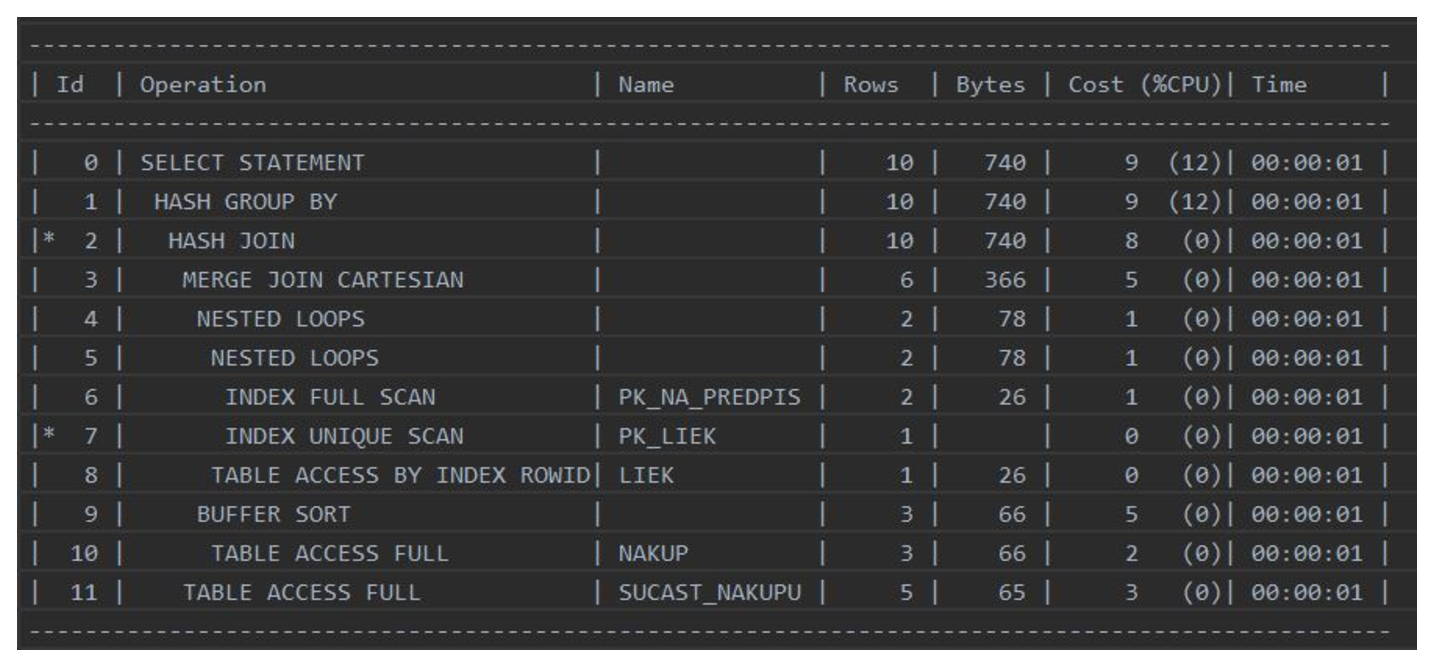
\includegraphics{bezIndexov.eps}}
	\centering
	\caption{EXPLAIN PLAN bez použitia indexov}
	\end{figure}

        \subsubsection{INDEX}
        K~urýchleniu prevedenia príkazu bol použitý príkaz INDEX nakoľko indexovanie môže byť užitočné v~prípade častého vyhľadávania v~určitej tabuľke. V~našej implementácií často používame tabuľky \texttt{LIEK} a \texttt{SUCAST\_NAKUPU}. 
        Preto sme implementovali príkazy INDEX nasledovne: \newpage
    \begin{lstlisting}
    CREATE INDEX sucast_index ON SUCAST_NAKUPU (ID_TABLE, NAKUP_ID, LIEK_ID);
    CREATE INDEX nakup_index ON NAKUP (CISLO_POKLADNICNEHO_BLOKU, DATUM_PREDAJA, LEKAREN);
    \end{lstlisting}
	\begin{figure}[h]
		\scalebox{0.6}{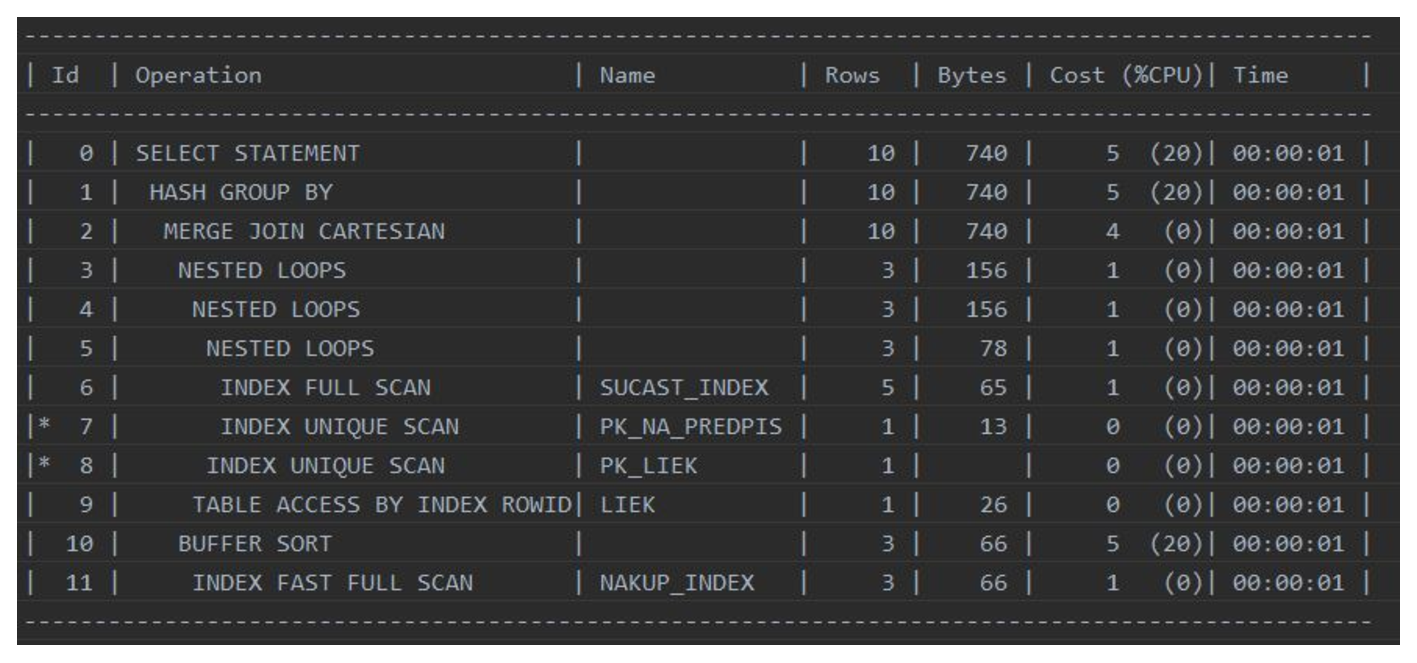
\includegraphics{sIndexami.eps}}
		\centering
		\caption{EXPLAIN PLAN s použitím indexov}
	\end{figure}
        Pri druhom spustení príkazov s~EXPLAIN PLAN za použitia indexov je viditeľné, že operácie sa vykonali rýchlejšie s~menšou výkonnostnou cenou. Taktiež miesto prechodu celou tabuľkou bolo zvolené skenovanie indexov. Táto zmena zabezpečila rýchlejšie/nenáročnejšie vykonanie väčšiny operácií v rámci príkazu.
	
	\subsection{Pocedúry} 
	Vytvorili sme dve procedúry:\\
	\texttt{percenta\_lieku\_z\_kapacity}\\
 	\texttt{volne\_miesto\_v\_sklade}\\
	
	Procedúra \texttt{percenta\_lieku\_z\_kapacity(sklady\_id\_arg)} počíta koľko percent liekov je na sklade s~ID v~parametri \emph{sklad\_id\_arg} z~celkového počtu liekov nachádzajúcich sa vo všetkých skladoch. Procedúra teda prechádza všetkými skladmi v~databáze a postupne počíta celkový počet liekov a počet ukladá do premennej \emph{pocet\_vsetkych\_liekov} ak sa spracováva sklad s~primárným kľúčom zhodným 
s~\emph{sklad\_id\_arg}, vtedy sa zároveň počet liekov ukladá do premennej \emph{lieky\_sklad}. Následne sa spočítajú percentá a daný výsledok sa s~presnosťou na dve desatinné miesta vypíše na DBMS výstup. V~prípade, že sklady sú prázdne, teda počet liekov je rovný 0, vyvolá sa výnimka.\\
	
	Procedúra \texttt{volne\_miesto\_v\_sklade} postupne zisťuje dostupnú kapacitu vo všetkých skladoch. Procedúra neprijíma nijaké parametre. Prehľadáva jednotlivé sklady a do premennej \emph{dostupna\_kapacita} zapisuje dostupnú kapacitu. Túto informáciu pre každý sklad potom vypíše na DBMS výstup. V~prípade, že by nejaký sklad bol plne obsadený, teda má dostupnú kapacitu 0, procedúra sa skončí s~chybou.

	\subsection{Materializovaný pohľad}
	Je to objekt, ktorý poskytuje dáta v~rovnakej podobe ako tabuľka. Narozdiel od tabuľky, ktorá obsahuje priamo dáta, pohľad obsahuje len predpis akým spôsobom dáta získať z~iných tabuliek alebo pohľadov. Materializovaný pohľad sa niekam ukladá a preto je dotaz rychlejší, čo neplatí o~nematerializovanom pohľade. \\
	\par Náš materializovaný pohľad vytvára tabuľku \texttt{mesta\_lekarni}, ktorá vytvára dáta okamžite a obnovuje ich pri commite. Následne je povolený prepis obsahu pohľadu. Pri demonštrácii je najprv vypísaný pôvodný pohľad, ktorý zobrazuje mestá, v~ktorých sa lekárne nachádzajú a ich počet v~danom meste. Potom vložíme nové dáta pomocou INSERT a vykonáme commit. Pri následujúcom výpise pomocou príkazu SELECT v~pohľade uvidíme aktualizované dáta.

	\subsection{Práva}
	Pomocou príkazu GRANT na tabuľky, potom následuje zoznam práv, ktoré povoľujeme (napr. INSERT, DELETE,...), ten sme zvolili ako ALL (všetky práva). Následujú názvy tabuliek, na ktoré chceme udeliť práva (opäť všetky tabuľky) a na koniec treba uviesť, komu sa tieto práva prideľujú, čo v~našom prípade bol kolega \textit{xbobos00}.

	\section{Záver}
	Pri vypracovaní projektu sme nemali žiadne závažné problémy v~komunikácii, keďže už sme zohratá dvojica a prácu sme si rozdelili rovnomerne. Projekt sme mali vypracovaný relatívne včas, aby sme sa vyhli zbytočným stresom pred deadline a prípadným preťaženiam školského servera, ako to býva zvykom pár dní pred odovzdávaním projektov. Vývoj projektu prebiehal na školskom serveri v~prostredí od JetBrains \-- Data Grip.
	\par Jedinou nevýhodou respektíve \uv{prekážkou} bola súčasná situácia vo svete a obmedzenie kontaktnej formy štúdia. Nemohli sme niektoré nejasnosti konzultovať s~pedagógmi a to spravilo prácu na projekte značne ťažšou.

\end{document}